\documentclass[11pt,letterpaper]{article}
\usepackage[margin=0.9in]{geometry}
\usepackage[T1]{fontenc}
\usepackage{lmodern,microtype}
\usepackage{amsmath,amssymb,bm,mathtools}
\usepackage{graphicx,booktabs,longtable,tabularx,array}
\usepackage{xcolor,enumitem}
\usepackage[most]{tcolorbox}
\usepackage[numbers,sort&compress]{natbib}
\usepackage{fancyhdr}
\usepackage{hyperref}
\definecolor{ink}{HTML}{215A78}
\definecolor{accent}{HTML}{D77A2B}
\hypersetup{colorlinks=true,linkcolor=ink,citecolor=ink,urlcolor=ink,pdftitle={Reading and follow-up analysis of arXiv:2412.00618},pdfauthor={Research planning report}}
\setlist{itemsep=3pt,topsep=4pt}
\setlength{\parskip}{5pt}
\setlength{\parindent}{0pt}
\setlength{\emergencystretch}{2em}
\renewcommand{\arraystretch}{1.15}
\newcolumntype{Y}{>{\raggedright\arraybackslash}X}
\newcommand{\R}{\mathbf R}
\newcommand{\rr}{\mathbf r}
\newcommand{\ee}{\mathrm e}
\newcommand{\ii}{\mathrm i}
\newcommand{\EC}{E_{\mathrm C}}
\newcommand{\LLL}{\mathrm{LLL}}
\newcommand{\avg}[1]{\left\langle #1\right\rangle}
\newtcolorbox{takeaway}{colback=ink!5,colframe=ink,boxrule=0.5pt,arc=2pt,left=8pt,right=8pt,top=5pt,bottom=5pt}
\pagestyle{fancy}
\fancyhf{}
\fancyhead[L]{\small arXiv:2412.00618 --- reading and follow-up}
\fancyhead[R]{\small 19 October 2026}
\fancyfoot[C]{\thepage}
\setlength{\headheight}{14pt}
\setcounter{tocdepth}{1}
\title{\textbf{Neural wavefunctions for the fractional quantum Hall problem}\\[6pt]\Large Detailed reading of arXiv:2412.00618\\and a practical follow-up research plan}
\author{Prepared for the Applied Machine Learning final-project workspace}
\date{19 October 2026}
\begin{document}
\maketitle

\begin{takeaway}
\textbf{Recommendation.} Use this paper as the physics foundation for a small, controlled study of \emph{when a learned complex wavefunction can be trusted}. For the course, make wavefunction prediction and its failure analysis the guaranteed deliverable; make unprojected Landau-level-mixing VMC a gated extension. For a longer research project, investigate mixing and competing phases in one validated moir\'e Hamiltonian with explicit topology and finite-size checks.

The central question proposed here is: \emph{Can good global fidelity or energy hide incorrect short-distance correlations, phase winding, or angular-momentum content, particularly on held-out physical conditions?} This is a hypothesis to test, not a result or a claim of established novelty.
\end{takeaway}

\textbf{What was read.} The complete local 17-page \texttt{2412.00618v2.pdf}, including the supplement and its training table; the local \texttt{Ghosh Term Project Applied ML.pdf}; and selected primary follow-up sources checked online through the report date. The local PDF and the journal title are \emph{Solving the fractional quantum Hall problem with self-attention neural network}, by Yi Teng, David D. Dai, and Liang Fu, \emph{Phys. Rev. B} \textbf{111}, 205117 (2025). The arXiv landing page instead uses \emph{Solving and visualizing fractional quantum Hall wavefunctions with neural network}. Both identify the same work. Paper page, section, equation, and figure numbers below refer to the local v2 PDF.\cite{teng}

\textbf{Status of this report.} Paper numbers are attributed reproductions of published results. Derivations and proposed protocols are analysis. No ED calculation, neural-network training, phase-boundary measurement, or runtime benchmark was performed for this report. The original schematic illustrates an analytic polynomial and is explicitly not numerical evidence about a trained state.

\newpage
\tableofcontents
\newpage

\section{The paper's argument in one connected outline}
\label{sec:outline}

\begin{longtable}{>{\raggedright\arraybackslash}p{0.16\linewidth}>{\raggedright\arraybackslash}p{0.37\linewidth}>{\raggedright\arraybackslash}p{0.39\linewidth}}
\toprule
Part and pages & What the authors do & What to retain when following up \\
\midrule\endhead
I, pp. 1--2 & Motivate continuum neural variational Monte Carlo (NN-VMC) for strongly correlated states beyond small projected Hilbert spaces. & The scientific target is a many-body complex wavefunction. It is not ordinary regression of energy from a few material parameters. \\
II, p. 2 & Contrast Laughlin's state with the Coulomb ground state; discuss relative-angular-momentum mixing and limitations of ED, DMRG, and fixed-phase DMC. & Separate errors in a trial state, LL projection, finite size, and optimization. Those errors have different remedies. \\
III, pp. 2--3; Fig. 1 & Construct a complex Psiformer wavefunction from generalized orbitals, determinant sums, Gaussian envelopes, and a real Jastrow factor. & Exchange antisymmetry is enforced. Laughlin correlations, angular-momentum sector, and topological order are learned rather than explicitly imposed. \\
IV, pp. 3--4 & Derive the Coulomb coalescence cusp and explain why an LLL-only function cannot represent it exactly. & Nonanalytic cusp and splitting of cubic zeros are different phenomena. Only the former necessarily requires LL mixing. \\
V, pp. 4--5; Fig. 2 & Define a finite neutralized electron droplet; minimize its variational energy with MCMC and KFAC; monitor angular momentum. & Background geometry, energy constants, gauge, and sampling uncertainty must match in any benchmark. \\
VI, pp. 5--6; Figs. 3--4 & Compare weak-mixing energies with LLL ED, show density and phase maps, and resolve linear versus cubic short-distance behavior. & The comparison changes the variational space. Frozen-coordinate phase plots reveal local structure, not a Hall conductance. \\
VII, pp. 6--8; Fig. 5 & Increase mixing, find excess kinetic energy and a different angular momentum and shell structure at strong mixing. & Evidence establishes a finite-droplet rearrangement; the thermodynamic crystal interpretation needs further diagnostics. \\
VIII, p. 8 & Propose crystals, Hall crystals, even-denominator states, and moir\'e applications. & Several of these directions already have direct 2025--2026 follow-ups; update the novelty assessment. \\
Supplement, pp. 11--17 & Give architecture, cusp discussion, potential interpolation, angular-momentum estimator, density plots, hyperparameters, and ED-sector definition. & This is required reading for reproduction. Important implementation choices remain unspecified or ambiguous. \\
\bottomrule
\end{longtable}

The argument is therefore: a flexible complex fermionic ansatz can optimize both amplitude and phase directly in the continuum; avoiding an explicit LL cutoff exposes correlation corrections missed by an LLL benchmark; the learned state can then be inspected in configuration space. Its most useful follow-up is to determine which physical conclusions survive stricter convergence, sampling, geometry, and topology tests.

\section{Physical problem, conventions, and controlled limits}
\label{sec:physics}

\subsection{What is actually being solved?}

There are $N$ fully spin-polarized electrons on an infinite two-dimensional plane, a uniform perpendicular magnetic field, and a fixed positive disk carrying charge $+Ne$. The disk has radius $a$ and lies at height $d$ above the electrons. Its potential confines a droplet, but there is no hard-wall boundary at $r=a$. The calculations use nominal filling $\nu=1/3$, with
\begin{equation}
 \ell_B=\sqrt{\frac{\hbar}{e|B|}},\qquad
 \omega_c=\frac{e|B|}{m^*},\qquad
 \EC=\frac{e^2}{4\pi\epsilon_0\epsilon\ell_B},\qquad
 \lambda=\frac{\EC}{\hbar\omega_c}.
 \label{eq:scales}
\end{equation}
Here $m^*$ is the mass of the modeled carriers; the paper writes atomic units with the mass set to one. The nominal density is fixed by disk flux:
\begin{equation}
 \pi a^2 B_{\rm abs}=\frac{N\Phi_0}{\nu},\qquad
 \frac a{\ell_B}=\sqrt{\frac{2N}{\nu}}=\sqrt{6N},\qquad
 \frac d{\ell_B}=0.1.
 \label{eq:disk}
\end{equation}
This finite-disk flux prescription is not the spherical shift relation $N_\phi=3(N-1)$ and does not make every finite-droplet density exactly uniform.

The approximations are fixed spin polarization, strictly two-dimensional carriers, a parabolic continuum dispersion, static dielectric screening represented by $\epsilon$, and a prescribed background. Spin transitions, finite transverse thickness, disorder, gates with a different screening kernel, and a microscopic lattice are outside this Hamiltonian. Avoid interpreting its strong-mixing state as a material-specific prediction before adding and validating those effects.

\subsection{One consistent gauge for reproduction}

The sign convention deserves an explicit decision. Take $z=x+\ii y$, canonical $L_z=-\ii\hbar(x\partial_y-y\partial_x)$, and choose the field orientation so holomorphic LLL orbitals have positive $L_z$. In units $\rr=\ell_B\mathbf x$, write
\begin{equation}
 \mathbf a(\mathbf x)=\tfrac12(y,-x),\qquad
 \hat T=\frac12\sum_i[-\ii\nabla_i+\mathbf a(\mathbf x_i)]^2
 =\sum_i\left[-\frac12\nabla_i^2+\frac{r_i^2}{8}-\frac{L_{z,i}}2\right].
 \label{eq:gauge}
\end{equation}
All operators in the last expression are dimensionless. Then $z^m\exp(-|z|^2/4)$ has kinetic energy $1/2$ and angular momentum $m$. This is the chirality used for positive Laughlin $M$ in this report.

With the paper's written minimal coupling $-\ii\nabla+\mathbf B\times\rr/2$, taking $B_z>0$ instead produces $+B_z L_z/2$ and favors antiholomorphic LLL orbitals. This is an orientation convention that must be fixed consistently, not a change in the underlying physics. A reproduction should test one known orbital before training; combining the positive-$M$ polynomial with the opposite signed vector potential silently invalidates the benchmark.

\subsection{Dimensionless Hamiltonian and background}

With $\tilde a=a/\ell_B$, $\tilde d=d/\ell_B$, and all coordinates below dimensionless, a convenient expression is
\begin{align}
 \frac H{\hbar\omega_c}&=\hat T+\lambda\hat V,\label{eq:dimlessH}\\
 \hat V&=\sum_{i<j}\frac1{|\mathbf x_i-\mathbf x_j|}
 +\sum_i v_c(\mathbf x_i)+v_b,\\
 v_c(\mathbf x)&=-\frac N{\pi\tilde a^2}
 \int_{|\mathbf x'|<\tilde a}\frac{d^2x'}{\sqrt{\tilde d^2+|\mathbf x-\mathbf x'|^2}},\qquad
 v_b=\frac{8N^2}{3\pi\tilde a}.
 \label{eq:background}
\end{align}
The self-energy $v_b$ shifts absolute energies but not the optimized state. It must nevertheless match in reported energy comparisons. The dielectric factor appears once through $\lambda$; the supplement's potential expression sets $\epsilon=1$, so inserting both an extra dielectric factor and $\lambda$ would double count screening.

The model depends only on $N$ and $\lambda$ after fixing $\nu$, $d/\ell_B$, and the geometry. Varying $d/\ell_B$ creates another physical control parameter. Varying laboratory $B$ while holding physical $d$ fixed also changes $d/\ell_B$; it is not the same path as varying only $\lambda$ in Eq.~\eqref{eq:dimlessH}.

\subsection{Why LLL projection is controlled only at weak mixing}

The unperturbed cyclotron spectrum is $(n+1/2)\hbar\omega_c$. For $\lambda\ll1$, projecting interactions into $n=0$ is the leading approximation. A schematic elimination of higher LLs gives
\begin{equation}
 H_{\rm eff}=P H P-P V Q\,(QH_0Q-E)^{-1}Q V P+\cdots,
 \label{eq:schur}
\end{equation}
where $V$ here denotes the dimensional interaction including the background and $Q=1-P$. The leading virtual correction is of order $\EC^2/(\hbar\omega_c)$ in absolute energy, or order $\lambda$ in Coulomb units. For an isolated weak-coupling branch, excited-LL amplitudes begin at order $\lambda$, and their occupation and kinetic excess begin at order $\lambda^2$ in cyclotron units. These are perturbative checks, not a justification for extrapolating a truncated expansion to $\lambda=3$ or $9$.

\section{Neural architecture: what is represented and what is imposed}
\label{sec:network}

\subsection{Generalized determinants and attention}

A usual Slater determinant uses orbitals $\phi_a(\rr_j)$ of one electron. A generalized determinant uses orbitals $\Phi_a(\rr_j;\R)$ depending on the full configuration $\R=(\rr_1,\ldots,\rr_N)$. Its rows or columns must transform consistently under relabeling electrons, while the distinguished electron's environment is otherwise represented without dependence on an arbitrary ordering. Exchanging two particles then exchanges two determinant rows or columns and gives the required minus sign.

The paper uses
\begin{equation}
 \Psi_\theta(\R)=\ee^{J_\theta(\R)}
 \sum_{k=1}^{K}\det\left[\Phi^{(k)}_{a}(\rr_j;\R)\right],\qquad
 J_\theta=-\beta\sum_{i<j}\frac{\alpha^2}{\alpha+r_{ij}}.
 \label{eq:ansatz}
\end{equation}
The orbitals have separately generated real and imaginary components and isotropic Gaussian envelopes. The sum of determinants improves flexibility; it is not a truncated expansion in a specified number of Landau levels. The Jastrow factor here is real and positive after exponentiation. It differs from Laughlin's complex polynomial pair factor.

For an electron token $h_i$, attention constructs queries, keys, and values and mixes other electrons' features. The standard scaled attention convention is
\begin{equation}
 q_i=W_qh_i,\quad k_j=W_kh_j,\quad v_j=W_vh_j,\qquad
 u_i=\sum_j\operatorname{softmax}_j\left(\frac{q_i^\mathsf T k_j}{\sqrt{d_h}}\right)v_j.
 \label{eq:attention}
\end{equation}
Shared weights and the sum over tokens preserve permutation equivariance. Stacked attention and MLP blocks learn collective environmental dependence. In this implementation, one-electron inputs enter attention, while pair distances explicitly enter the Jastrow factor. The figure's mention of two-electron features should not be read as a FermiNet-style pair stream inside every attention layer.\cite{psiformer}

The supplement's printed attention scaling differs from Eq.~\eqref{eq:attention}: it places a factor outside the softmax. Code should follow a verified implementation or explicitly document a deliberate alternative. This is a reproducibility issue because rescaling logits and rescaling attention outputs are different operations.

\subsection{Meaning and limits of the ansatz}

The determinant does not restrict this state to Hartree--Fock: each matrix element depends on all particles, so the resulting function can contain correlations far beyond one-body orbitals. Conversely, a finite network trained for finite time is not an exact treatment of the full Hilbert space. It avoids an \emph{explicit LL cutoff}, but retains representation, optimization, sampling, precision, and finite-size errors.

The architecture contains substantial physical structure: fermionic antisymmetry, fixed spin polarization, normalizable Gaussian tails, and a Coulomb-motivated pair factor. What it does not explicitly encode is the Laughlin polynomial, the desired angular momentum, or the phase it should discover. This distinction is more precise than calling it completely free of prior physics.

At fixed width and depth, attention has an $N^2$ token interaction cost, while determinants typically have an $N^3$ linear-algebra cost per determinant. Kinetic energy requires spatial second derivatives; those can dominate actual runtime and memory. A polynomial cost per network evaluation does not establish polynomial total cost for reaching a fixed physical accuracy as $N$ increases.

\section{Coulomb cusp, zero splitting, and what each tells us}
\label{sec:cusp}

\subsection{A short independent derivation of the cusp}

Near two equal-mass particles, set $\rr=\rr_1-\rr_2$, $\mathbf R_{\rm cm}=(\rr_1+\rr_2)/2$. In atomic units the singular part of the relative Hamiltonian is
\begin{equation}
 H_{\rm rel}=-\nabla_{\rr}^2+\frac1{\epsilon r}+\text{terms regular at }r=0.
\end{equation}
For a component of relative angular momentum $l$, let
\begin{equation}
 \psi_l(r,\varphi)=\ee^{\ii l\varphi}r^{|l|}(1+c_l r+O(r^2)).
\end{equation}
In two dimensions,
$\nabla^2(r^{s+1}\ee^{\ii l\varphi})=(2s+1)r^{s-1}\ee^{\ii l\varphi}$ for $s=|l|$.
Cancellation of the leading singular term yields
\begin{equation}
 c_l=\frac1{\epsilon(2|l|+1)}\quad\text{in atomic-length coordinates},\qquad
 c_l^{(\ell_B)}=\frac{\lambda}{2|l|+1}\quad\text{in magnetic-length coordinates}.
 \label{eq:cusp}
\end{equation}
For identical spin-polarized particles, $l$ is odd. A generic nonzero $|l|=1$ component dominates sufficiently near coalescence and has coefficient $\lambda/3$ in the dimensionless convention. The $|l|=3$ component has coefficient $\lambda/7$.

This direct singular-term argument avoids apparent algebraic transcription problems in intermediate supplementary equations. For example, the center-of-mass and relative Laplacian coefficients in its Eq.~S8 are inconsistent with the stated coordinates; the standard transformation gives $-\nabla_{\rr}^2-\frac14\nabla_{\mathbf R_{\rm cm}}^2$. The final cusp coefficient in main Eq.~4 is nevertheless consistent with the independent derivation above.

\subsection{What the chosen pair factor actually enforces}

For one pair, the paper's exponent has expansion
\begin{equation}
 -\beta\frac{\alpha^2}{\alpha+r}=-\beta\alpha+\beta r+O(r^2).
\end{equation}
Thus its pair factor supplies a linear radial slope $\beta$. The practical value $\beta=1/4$ at $\epsilon=1$ interpolates between $1/3$ and $1/7$; it is not the exact asymptotic $l=1$ cusp coefficient. Main-text language treats $\beta$ as initialized/trainable, while supplementary Eqs.~S6 and S17 emphasize trainable $\alpha$ with a fixed $1/4$. A reproduction must declare which interpretation is used.

Do not carry $1/4$ unchanged into dimensionless calculations over $\lambda$. Its corresponding heuristic slope scales as $\lambda/4$, while a pure $l=1$ exact slope is $\lambda/3$. Also, a prefactor only enforces the complete cusp if the residual network introduces no additional competing nonanalytic slope. A learned dependence on $r_{ij}$ can change that slope. Check the measured total wavefunction, not only the written Jastrow term.

\subsection{Why cusp requires higher LLs but split zeros do not}

An LLL state has the form
\begin{equation}
 \Psi_{\LLL}=f(z_1,\ldots,z_N)\exp\left(-\sum_i\frac{|z_i|^2}{4\ell_B^2}\right),
\end{equation}
with $f$ holomorphic and antisymmetric. Finite LL expansions add analytic polynomials in $z$ and $\bar z$ times Gaussians. They cannot reproduce the exact nonanalytic $|z_{12}|$ cusp at arbitrarily small separation; its exact representation requires infinitely many LLs. Practical convergence at finite resolution is still possible with finite resources.

By contrast, an LLL Coulomb state can already contain both relative $l=1$ and $l=3$. Locally, after fixing the other variables suitably,
\begin{equation}
 \psi\simeq A z+Bz^3=Bz(z-\xi)(z+\xi),\qquad \xi^2=-A/B.
 \label{eq:zeros}
\end{equation}
The Pauli zero remains at coincidence, while two additional zeros move away. This function is holomorphic. Consequently, \textbf{observing a split cubic zero does not by itself demonstrate LL mixing}. The excess kinetic energy and nonanalytic cusp provide different evidence.

\begin{figure}[htbp]
\centering
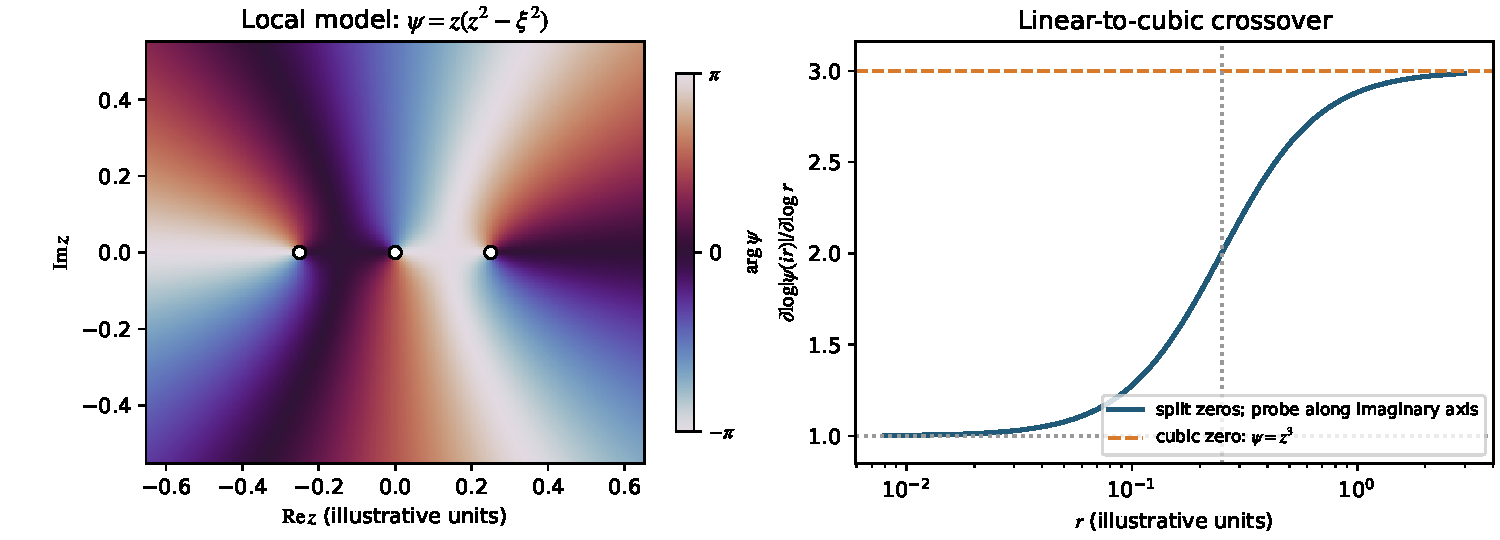
\includegraphics[width=\linewidth]{fqh_zero_splitting_schematic.pdf}
\caption{Original analytic illustration, not a neural or ED result. For $\psi=z(z^2-\xi^2)$ with $\xi=0.25$ in illustrative units, each simple zero has unit phase winding. Along $z=\ii r$, $|\psi|=r(r^2+\xi^2)$ and the logarithmic slope is $1+2r^2/(r^2+\xi^2)$. It crosses from one to three without LL mixing. The full physical wavefunction also has Gaussian and environmental dependence.}
\label{fig:schematic}
\end{figure}

\subsection{What to measure instead of relying on a single picture}

A phase map freezes $N-1$ coordinates and moves the last. It is a conditional configuration-space slice, not the one-body reduced density matrix or the marginal electron density. The paper selects the highest-probability configuration among 5000 samples. That is a useful illustration but not a representative statistical average; analyze many independent frozen configurations and report a distribution of zero separations and local slopes.

For a loop $C$ avoiding zeros, estimate integer winding from wrapped phase increments:
\begin{equation}
 w(C)=\frac1{2\pi}\sum_k\operatorname{Arg}\left[\Psi(\R_{k+1})\Psi(\R_k)^*\right].
\end{equation}
Refine the loop mesh and reject paths where amplitudes are too small for stable phase evaluation. The unit or triple winding in such a slice is not a quasihole exchange Berry phase or a many-body Chern number. A smooth, single-valued gauge transformation leaves these local integer windings unchanged, while the displayed absolute phase colors remain gauge dependent.

For a stricter pair-angular-momentum diagnosis, vary the relative angle at fixed pair center of mass and fixed spectators, and Fourier analyze the complex wavefunction. Moving just one electron also moves the pair center of mass, mixing environmental variation into the apparent local power. The linear-trimer picture is a leading local model, not a universal exact constraint on every finite configuration.

\section{Variational learning and trustworthy estimators}
\label{sec:vmc}

\subsection{Loss and gradient for a complex wavefunction}

The probability measure is the joint $2N$-dimensional configuration density
\begin{equation}
 p_\theta(\R)=\frac{|\Psi_\theta(\R)|^2}{\int d\R\,|\Psi_\theta(\R)|^2},\qquad
 E(\theta)=\avg{E_L}_{p_\theta},\quad E_L=\frac{H\Psi_\theta}{\Psi_\theta}.
\end{equation}
It should not be confused with the one-body density $\rho(\rr)$, which is a marginal of this distribution. For real parameters and a parameter-independent Hermitian $H$,
\begin{equation}
 \partial_{\theta_a}E=2\operatorname{Re}\avg{(E_L-E)O_a^*},\qquad
 O_a=\partial_{\theta_a}\log\Psi_\theta.
 \label{eq:gradient}
\end{equation}
The normalization derivative is included in the covariance form. A generic backpropagation through a fixed batch of mean local energies is not automatically this variational gradient. Verify the estimator independently before comparing optimizers.

Write $u=\log\Psi$ locally away from zeros. For $\nabla\cdot\mathbf a=0$, the dimensionless kinetic local energy is
\begin{equation}
 T_L=-\frac12\sum_i\left[\nabla_i^2u+(\nabla_i u)\cdot(\nabla_i u)\right]
 -\ii\sum_i\mathbf a_i\cdot\nabla_i u+\frac12\sum_i\mathbf a_i^2.
 \label{eq:localT}
\end{equation}
The dot product in the squared complex gradient has no complex conjugation. Use stable complex log-determinant evaluation and derivative formulas; differentiating a wrapped phase image creates artificial discontinuities. The integrated energy is real, but local energies may be complex; check that their imaginary mean is statistically consistent with zero.

\subsection{Why energy and mean angular momentum are insufficient}

A variational state satisfies $E\ge E_0$ for the exact same Hermitian Hamiltonian in expectation. A noisy estimate can fall below it, and interpolation changes the Hamiltonian being evaluated. Likewise, $\operatorname{Var}(H)=0$ identifies an eigenstate, including an excited eigenstate. A small variance can coexist with an inaccurate state when nearby levels are dense.

For a normalized state and a known nonzero gap $\Delta=E_1-E_0$, one can bound its ground-state weight by
\begin{equation}
 1-|\avg{\Psi_0|\Psi}|^2\le\frac{E-E_0}{\Delta}.
\end{equation}
Without a reliable gap and reference energy this is not a practical certification. Small edge gaps make a small energy error especially weak evidence of high fidelity.

For $\hat M=\sum_i-\ii(x_i\partial_{y_i}-y_i\partial_{x_i})$, define $M_L(\R)=\hat M\Psi/\Psi$. Report both
\begin{equation}
 \avg M=\avg{M_L},\qquad
 \operatorname{Var}(M)=\avg{|M_L|^2}-|\avg{M_L}|^2.
 \label{eq:Mvar}
\end{equation}
The squared modulus uses the full complex local value. The variance of only $\operatorname{Re}M_L$ is not a substitute. An equal superposition of sectors $M_0-1$ and $M_0+1$ has integer mean $M_0$ and variance one. Even a circular one-body density can hide an incoherent or coherent mixture with inappropriate sector content. Conversely, a genuine angular-momentum eigenstate has circular one-body density, including a rotating Wigner molecule.

\subsection{Sampling and error bars}

Use independently initialized chains, discard burn-in, and estimate integrated autocorrelation for energy and for slower observables such as shell occupancy and phase-related quantities. If $\tau_{\rm int}=1+2\sum_{k\ge1}\rho_k$, then $n_{\rm eff}\simeq n/\tau_{\rm int}$. State the convention because some definitions differ by a factor of two. Blocking or a chain-level bootstrap should agree with the estimated uncertainty when blocks are long enough.

Re-equilibrate and evaluate a frozen final checkpoint on new chains. Training fluctuations mix parameter drift with MCMC noise and do not provide a valid final error bar. Monitor acceptance, cross-chain agreement, and node-adjacent tails. Near-coalescence configurations are strongly suppressed by Fermi statistics, so nominally large sample counts can still contain almost no information about the cusp or the smallest split zeros.

Keep unclipped final physical estimators. Robust clipping can stabilize training but changes its effective objective and should be reported. Distinguish Monte Carlo uncertainty, seed-to-seed optimization variability, numerical quadrature error, and model/truncation bias; combining them into one unexplained parenthesis obscures the reliability question.

\section{Results in the paper: evidence and its limits}
\label{sec:results}

\subsection{Weak mixing and the ED comparison}

Figure 3(a), on PDF p.~5, reports the following total energies per electron in Coulomb units at $\lambda=1/3$. The table is transcribed from the figure; these are not newly computed values.

\begin{center}
\begin{tabular}{rrrrr}
\toprule
$N$ & Neural $E/(N\EC)$ & LLL ED $E/(N\EC)$ & ED minus neural & LLL sector dimension\\
\midrule
6 & 1.1372(4) & 1.13836 & 0.00116 & 1,206\\
7 & 1.1357(4) & 1.13687 & 0.00117 & 8,033\\
8 & 1.1347(2) & 1.13588 & 0.00118 & 55,974\\
9 & 1.1346(1) & 1.13545 & 0.00085 & 403,016\\
10 & 1.1342(4) & 1.13496 & 0.00076 & 2,977,866\\
11 & 1.1337(4) & --- & --- & 22,464,381\\
12 & 1.1334(3) & --- & --- & 172,388,026\\
\bottomrule
\end{tabular}
\end{center}

ED is actually performed only through $N=10$. The final two dimensions indicate the growth of the LLL sector, not completed ED benchmarks. The ED space contains all LLL determinants at total $M=M_{\rm Laughlin}=3N(N-1)/2$, with no additional imposed single-orbital cutoff. At fixed $M$ and nonnegative orbital labels, the allowed set is already finite.

The defensible comparison is
\begin{equation}
 E_0^{\rm full}\le E_{\rm VMC}^{\rm full},\qquad
 E_0^{\rm full}\le E_{\rm ED}^{\LLL,M_{\rm Laughlin}}.
\end{equation}
There is no theorem ordering the two approximate values. A reliably smaller unrestricted VMC energy demonstrates an improvement over the specified restricted benchmark. If the neural state is in the same $M$ sector, it also demonstrates LL content beyond that sector's LLL minimizer. If sector purity is not established, a lower value could partly reflect a different sector. Excess kinetic energy is a cleaner direct mixing diagnostic.

For $N=10$, the reported difference $0.00076$ is about 1.9 times the quoted neural error unit $0.0004$; therefore one should not describe every individual weak-mixing entry as overwhelming statistical evidence without knowing the uncertainty procedure. The paper gives useful consistency across sizes, but a follow-up should state confidence intervals and systematic errors explicitly.

At $\lambda=1/3$, the LLL kinetic energy is $\hbar\omega_c/(2\EC)=1.5$ per electron in Coulomb units. Subtracting it turns the positive total energies above into negative reduced electrostatic-plus-mixing energies. Confusing these two reporting conventions produces an apparent order-one disagreement.

\subsection{What the density and phase maps establish}

The $N=12$ neural state gives $\avg M=197.97$, close to $M_{\rm Laughlin}=198$, and a nearly circular density. This supports successful learning of the expected sector and spatial symmetry. It does not measure its angular-momentum variance or provide a rigorous overlap with the full ground state.

Figure 4 shows local simple zeros and a crossover from linear to cubic behavior in a conditional wavefunction slice, unlike the exact cubic coincidence zeros of the Laughlin ansatz. This is valuable microscopic information. It does not isolate the fraction of that effect caused by LLL Coulomb corrections versus additional LL mixing. The clean follow-up comparison is Laughlin versus converged LLL Coulomb ED versus unrestricted VMC, all at the same $N$, background, and intended sector.

\subsection{Strong mixing and the interpretation of a new state}

Figure 5 uses $N=9$ and $\lambda=1/3,1,3,9$. At $\lambda=3$ and $9$, the kinetic energy visibly exceeds $\hbar\omega_c/2$ per electron. Define
\begin{equation}
 \bar n_{\rm LL}=\frac{\avg T}{N\hbar\omega_c}-\frac12.
 \label{eq:LLmeasure}
\end{equation}
For the parabolic kinetic operator this is the mean LL index per electron. It is nonnegative and vanishes for an exactly LLL state. It is not the probability that an electron is outside the LLL, since higher LLs carry different weights.

The observed angular momentum changes from $108$ for the first three mixing values to $100$ at $\lambda=9$. The cumulative radial density develops a plateau near one electron in the center and eight in the outer shell. Supplementary Fig.~S3 shows $N=10$ changing from $135$ to $127$, with two inner and eight outer electrons. These observations are consistent with shell ordering and a rotating Wigner-molecule interpretation.

For a finite rotationally symmetric droplet, this is evidence for a change in the optimized state and potentially a level crossing. Four widely spaced mixing values do not locate a critical coupling, determine the transition order, establish a thermodynamic Wigner crystal, or exclude an intervening Hall crystal. The paper itself discusses these qualifications on p.~8. A strong follow-up should preserve that distinction.

\begin{takeaway}
\textbf{The most useful conceptual separation.} Cubic-zero splitting tests departures from the Laughlin polynomial. The Coulomb cusp and excess kinetic energy test LL mixing. Angular-momentum purity tests symmetry content. A topological response or ground-state-manifold diagnostic tests topological order. No one of these substitutes for the others.
\end{takeaway}

\section{Reproduction audit and a minimal reliable implementation}
\label{sec:reproduce}

\subsection{Reported settings and unresolved choices}

Supplementary Table I gives two Psiformer layers, four heads, head dimension 64, layer width 256, KFAC, norm constraint and damping both $0.001$, initial learning rate $0.005$, delay $200000$, decay 1, batch size 6000, ten MCMC steps between updates, FP32, no input rescaling, and no layer normalization. Training mostly used four NVIDIA P100 GPUs or one A100. A smaller-system suggestion is learning rate $0.02$ with delay $20000$. The authors report precision-dependent instability involving TF32.

These facts do not specify a complete reproduction recipe. Missing or unclear items include determinant count, parameter count, exact total updates and stopping rule, learning-rate schedule implementation, random seeds, proposal kernel and tuned widths, warmup, separate final-evaluation length, checkpoint selection, and how reported statistical errors were estimated. The fixed-versus-trainable cusp parameter and the attention convention also need resolution. Do not infer hours or total GPU-days from the device list alone.

The paper cites the upstream FermiNet repository and JAX. A paper-specific runnable release and checkpoints were not established in the targeted search; that is not proof that none exist. Later torus code and WF-Bench have public repositories, but they implement different methods and should not be relabeled as the exact Teng et al. release.\cite{ferminetcode,fadoncoderef,wfbenchcode}

\subsection{Implementation sequence with concrete acceptance gates}

\begin{enumerate}
\item \textbf{Freeze units and conventions.} Store $N$, $\nu$, $d/\ell_B$, signed vector potential, $\lambda$, energy convention, and background normalization in a configuration file. The input coordinates and every potential term must use the same units.
\item \textbf{Verify the kinetic operator analytically.} Evaluate $z^m\ee^{-|z|^2/4}$ for several $m$; require local kinetic energy $1/2$ and $M=m$ away from numerical zeros. Verify finite differences and automatic derivatives on smooth points.
\item \textbf{Verify antisymmetry and normalization behavior.} Randomly exchange particles, requiring $\Psi(P\R)=-\Psi(\R)$ to numerical tolerance. Rotate a known Laughlin teacher, requiring phase $\ee^{\ii M\varphi}$ and invariant modulus. Check Gaussian tails and stable log determinants.
\item \textbf{Validate the disk potential independently.} Compare quadrature with an interpolation grid at center, near edge, and outside. The paper uses 10000 points to $15a$ and a far-field point-charge tail. Its claimed small pointwise relative error must be compared with the much smaller target energy differences. Relative potential accuracy alone does not establish enough total-energy accuracy.
\item \textbf{Use the exact same approximate potential on both sides.} Otherwise ED and VMC solve slightly different Hamiltonians. Refine the grid until the resulting energy difference is stable. A convex interpolation argument inside the disk does not by itself bound all outside-tail contributions or all implementation errors.
\item \textbf{Calibrate MCMC on an analytic teacher.} Confirm radial normalization $\int\rho\,d^2r=N$, known $M$, and identical results from independent chains and proposal scales. Inspect energy tails and $n_{\rm eff}$ before using the sampler for optimization.
\item \textbf{Start with $N=2$ or $3$.} Cross-check against an independent radial or systematically enlarged few-particle calculation. Then move to $N=4$ and only increase to $6$ if derivative cost, accuracy, and sampling gates pass.
\item \textbf{Add the neural state without changing the Hamiltonian.} Establish a small deterministic validation batch, correct complex variational gradients, and a stable optimizer. If replacing KFAC with Adam or SR, label it as a methodological change and compare total cost.
\item \textbf{Separate training from final measurement.} Freeze the checkpoint; start new chains; estimate $E$, $\operatorname{Var}(H)$, $\avg M$, $\operatorname{Var}(M)$, $\bar n_{\rm LL}$, density, and short-distance diagnostics. Retain failures and seed variability.
\end{enumerate}

\subsection{An apples-to-apples ladder of reference states}

Use, in order: the analytic Laughlin state; the exact LLL Coulomb state at fixed $M$; a systematically converged few-LL/few-particle reference where affordable; and the unrestricted neural ansatz. Compare the same $N$, potential, gauge, and energy constants. A separate scan over $M$ is needed to establish the global disk ground state. If ED is restricted to a chosen sector, label it accordingly.

The LLL basis at fixed $M$ is formed from distinct nonnegative integers $m_1<\cdots<m_N$ satisfying $\sum_i m_i=M$. Increasing an unnecessary orbital cutoff while keeping this sector fixed should not create new configurations once all such partitions are included. For higher LLs, specify both the cyclotron and guiding-center cutoffs and demonstrate convergence; a nominal LL count alone may not define a finite calculation.

\section{What has already been followed up by October 2026}
\label{sec:literature}

This is a targeted primary-source check, not an exhaustive citation review. It changes the project framing substantially. The original paper is a good starting point, but several obvious extensions are already established research directions.

\begin{enumerate}
\item \textbf{Physics-informed amplitude and current initialization.} Nazaryan, Gaggioli, Teng, and Fu, arXiv:2507.13322, first submitted July 2025, revised February 2026, learn complex states using configuration probability and probability current, then use pretraining for larger Coulomb FQH calculations. This is the direct starting point for phase-aware learning; generic Laughlin pretraining is not a new contribution.\cite{nazaryan}
\item \textbf{A general wavefunction learning benchmark.} Zhang, Duan, and Luo, \emph{WF-Bench}, arXiv:2605.29683, ICML 2026, supplies a broad benchmark organized around wavefunction fidelity and scaling. Its public code is a practical entry point. Before claiming a new sampling or architecture benchmark, compare its protocol with the proposed short-distance and held-out-interaction tests.\cite{wfbench,wfbenchcode}
\item \textbf{Torus liquid--crystal competition.} Abouelkomsan and Fu, arXiv:2602.03927, published in \emph{PRX Intelligence} \textbf{1}, 013010 (2026), introduce MagNet for magnetic torus states and study crystallization with LL mixing. Therefore simply removing the disk edge or locating a liquid--crystal transition on a torus is already a direct follow-up.\cite{magnet}
\item \textbf{Direct topological characterization.} Perez Fadon and collaborators, arXiv:2512.15872, published in \emph{PRX Intelligence} \textbf{1}, 013018 (2026), use neural torus ground states and entanglement interferometry to extract the modular $S$ matrix. This addresses a limitation of conditional phase plots. Reproducing such evidence is valuable but is not a novel proposal by itself.\cite{fadon}
\item \textbf{Physics-based composite-fermion backflow.} Gattu, arXiv:2512.00527, develops CF-Flow: symmetry-preserving neural dressing of composite-fermion states, with LL mixing and transport-gap calculations. A generic proposal to add physical trial states or backflow must be distinguished from this existing approach.\cite{gattu}
\item \textbf{Continuum moir\'e topological states.} Li and collaborators, arXiv:2503.11756, use neural wavefunctions for integer and fractional topological states in twisted MoTe$_2$. It is an especially relevant predecessor for the user's materials direction; applying a continuum network to a moir\'e system is not automatically new.\cite{limoire}
\item \textbf{Topology through momentum decomposition.} Abouelkomsan, Geier, and Fu, arXiv:2512.01863, published as \emph{Topological Order in Neural Wavefunctions}, \emph{Phys. Rev. B} \textbf{113}, 205119 (2026), develop topological ground-state-degeneracy diagnostics from optimized real-space states. This belongs in the reading path before proposing topology solely from density or one Chern-like number.\cite{deepstate}
\item \textbf{Even-denominator non-Abelian states.} Graham, Abouelkomsan, and Fu, arXiv:2610.18967, submitted 13 October 2026, report momentum-resolved neural calculations at $\nu=3/2$ with strong mixing and non-Abelian characterization. It is a very recent preprint, not an independently reproduced conclusion in this report. It makes a generic non-Abelian extension an unsuitable novelty claim.\cite{graham}
\item \textbf{An independent spherical-geometry study.} Qian and collaborators, arXiv:2412.14795, published in \emph{Phys. Rev. Lett.} \textbf{134}, 176503 (2025), investigate neural FQH states and LL mixing at $1/3$ and $2/5$ on a sphere. This provides an independent reference and removes a physical disk edge, with different finite-size geometry and flux conventions.\cite{qian}
\end{enumerate}

The accessible opportunity is a specific reliability, generalization, physical-assumption, or cost question that these works do not settle for the chosen setup. A controlled negative result can be a useful research contribution: for example, showing exactly when a high-fidelity learned state fails a short-distance observable and which additional diagnostic detects it. The actual novelty of that narrow question still requires a focused full-text comparison before publication claims.

\section{Recommended course-scale question and experimental design}
\label{sec:project}

\subsection{Question, hypotheses, and scientific contribution}

\textbf{Working title:} \emph{When can we trust a learned fractional quantum Hall wavefunction? Prediction of complex states and tests of short-distance reliability.}

\textbf{Primary question.} At fixed model and compute budgets, do global learning metrics predict correct short-distance phase and correlation structure when the physical interaction changes?

\textbf{Hypothesis H1.} A model can achieve high global fidelity while substantially misestimating rare close-pair behavior, because those regions have small probability mass. Phase-aware supervision and appropriately weighted close-pair examples may improve those observables per unit cost. This is not guaranteed: derivative labels can be noisy or singular and can destabilize learning.

\textbf{Hypothesis H2.} A reported integer $\avg M$ can hide sector contamination. Adding $\operatorname{Var}(M)$ and independent-chain validation changes which checkpoints are considered reliable, even if the best final energy changes little.

\textbf{Hypothesis H3, stretch.} A warm start learned near the Laughlin regime can reduce optimization cost at weak mixing yet bias finite-budget training when the target develops different correlations or a different angular momentum. Cold starts, both scan directions, and multiple sectors can reveal that failure.

The contribution is a reproducible physical reliability study with a defined distribution shift, not invention of attention, pretraining, mixed sampling, or a claim to discover FQH order for the first time. Pre-register the main observables and budgets before tuning.

\subsection{A teacher family that isolates one change}

For the guaranteed supervised component, fix $N=4$ initially, $\nu=1/3$, the disk geometry, and $M=M_{\rm Laughlin}$. Use an LLL teacher, so state explicitly that \emph{this stage studies deviations from Laughlin within one LL; it does not model the Coulomb cusp or LL mixing}. Construct
\begin{equation}
 H_{\rm teacher}(t)=(1-t)\sum_{i<j}P^{(ij)}_{l=1}
 +t\,P_0\left[\sum_{i<j}\frac1{r_{ij}}+\sum_i v_c(\rr_i)+v_b\right]P_0,
 \quad 0\le t\le1.
 \label{eq:teacher}
\end{equation}
The parent pseudopotential coefficient sets the unit of the first term; all terms in this synthetic interpolation are dimensionless in an explicitly chosen common energy unit. $P_{l=1}^{(ij)}$ penalizes relative pair angular momentum one. At $t=0$, the densest $\nu=1/3$ Laughlin state is the unique zero-energy state in the selected minimal sector. At $t=1$, the teacher is the projected Coulomb droplet in that sector. Background confinement is turned on with the Coulomb term so the parent endpoint remains exact. This is a joint Hamiltonian interpolation controlled by one parameter, not an attribution of changes solely to pair repulsion.

The interpolation parameter $t$ is a designed interaction change. It is \textbf{not} $\lambda$. An LLL teacher remains holomorphic at every $t$, so no amount of supervised accuracy can teach the genuine nonanalytic Coulomb cusp from these labels. This separation lets the project ask a precise question about zero splitting without confusing it with LL mixing.

Diagonalize the small fixed-sector matrix and evaluate the resulting Slater expansion and its derivatives at sampled coordinates. Validate the $t=0$ eigenvector against Laughlin and check hermiticity, normalization, and exact angular momentum before using the dataset. Start with roughly 12--20 teacher values of $t$, then add density only if label evaluation is affordable. A fixed small $N$ study has strong state-space coverage but limited physical-condition diversity; report both.

\subsection{Guaranteed fallback if a validated ED teacher is not ready}

First use analytic Laughlin states, which supply exact coordinate labels. For a controlled change of zero structure at the same $N$ and $M$, construct a second antisymmetric homogeneous LLL polynomial $\chi$ linearly independent of Laughlin, orthogonalize it with the Gaussian LLL inner product, and define normalized known states
\begin{equation}
 \Psi_t=\cos\alpha(t)\,\Psi_{\rm Laughlin}
 +\sin\alpha(t)\,\chi,\qquad \avg{\Psi_{\rm Laughlin}|\chi}=0.
 \label{eq:analyticteacher}
\end{equation}
A generic distinct Slater determinant at the same total $M$ provides a candidate before orthogonalization. Both basis functions must be normalized in the same convention. This is an exactly labeled representability and generalization stress test, \emph{not a claimed Coulomb ground-state path or physical phase transition}. If ED later passes validation, replace or supplement these labels with Eq.~\eqref{eq:teacher}. The fallback should not depend on completing an unprojected solver.

This family should also be a positive control even if ED succeeds. Its fidelity to Laughlin is exactly $\cos^2\alpha$, yet any nonzero coefficient of a generic $l=1$ state changes the asymptotic coincidence exponent from three to one. The logical possibility of high fidelity and a different asymptotic zero is therefore known analytically; the empirical research target is \emph{finite-resolution recovery, cost, and practical observable error}, not proving that possibility by training. Along a nonsingular local ray, the crossover scale is approximately $r_*\sim\sqrt{|A/B|}$ in Eq.~\eqref{eq:zeros}. Verify that $r_*$ lies inside the stated probe window before classifying a model's unresolved linear regime as a failure.

\subsection{The prediction task and training targets}

Inputs are the full coordinate configuration and, for a conditional model, $t$. A shared scalar condition can be appended to each token without breaking permutation equivariance. Outputs are a complex antisymmetric wavefunction, conveniently evaluated through a stable log-amplitude and complex phase representation. Raw phase regression with a discontinuous $[-\pi,\pi)$ target is a poor default.

Use teacher log-amplitude $a_*=\log|\Psi_*|$ and the probability velocity in the fixed gauge,
\begin{equation}
 \mathbf v_{*,i}=\frac{\mathbf j_{*,i}}{p_*}=\nabla_i\phi_*+\mathbf a_i,
 \qquad \phi_*=\arg\Psi_*.
\end{equation}
These are full configuration-space quantities. A one-body charge/current map is insufficient to determine a generic many-body state. The velocity here is inherited from the unprojected parabolic kinetic operator and is an auxiliary gauge-covariant supervision target for the LLL synthetic Hamiltonian; it is not automatically its conserved projected transport current. In the chosen dimensionless units a practical supervised objective is
\begin{equation}
 \mathcal L_A=\mathbb E_q[(a_\theta-a_*-c)^2],\qquad
 \mathcal L_{A+v}=\mathcal L_A+\eta\,\mathbb E_q\sum_i\|\mathbf v_{\theta,i}-\mathbf v_{*,i}\|^2,
 \label{eq:superloss}
\end{equation}
where $c$ removes the arbitrary additive log-normalization for each teacher condition. The weight $\eta$ is selected using validation data, with units and feature scales fixed. Phase gradients avoid global phase ambiguity, although disconnected nodal regions can still leave relative-phase ambiguities. Evaluate global fidelity as an additional check rather than assuming density and current determine every state uniquely.

Near nodes, $\nabla\log\Psi$ can diverge. Use a documented sampling distribution, finite label masks or smooth weights for training stability, and a separate uncensored physical evaluation wherever numerically resolvable. Report excluded mass and cutoff sensitivity. Derivative-based learning costs more than amplitude-only learning; comparisons must include that cost.

LLL analyticity locally relates log-amplitude and phase through the Cauchy--Riemann equations. Additional current labels therefore guide the unrestricted coordinate student's learning; they are not fundamentally independent physical information for a strictly holomorphic student. The coefficient baseline has that LLL constraint built in. Distinguish this difference in inductive structure from a comparison of loss terms within the same unrestricted architecture.

\subsection{Sampling distributions and leakage control}

Start with independent chains sampling $|\Psi_*|^2$. Add a clearly specified set of close-pair probes, spanning, for example, $r_{ij}/\ell_B$ from $0.02$ to $0.5$, with several angular directions and varied spectators. First select a spectator configuration, then generate all nearby pair probes. Every derivative, rotation, permutation, and close-pair variant descended from that configuration belongs to the same train/validation/test group.

There are two different objectives. Physical expectations are integrals under the physical density and require correct importance weights if evaluated with a different proposal. An intentionally reweighted rare-event training loss is a design choice; it does not itself estimate a physical expectation. If using a mixture proposal $q$, verify its density and support before constructing weights $p_*/q$. Correlated or unnormalized ad hoc probes can be used for a named stress test, but should not be passed off as unbiased samples of $p_*$.

Choose an interpolation test with entire omitted $t$ values and an extrapolation test holding out, for example, the upper interval $t\in[0.8,1]$. Tune only on training and validation conditions. New configurations at a seen $t$ test configuration generalization; unseen $t$ values test physical-condition generalization. They answer different questions. In each case keep independent sampler chains or chain blocks across partitions and estimate residual autocorrelation.

For $N=4$, 20000 configurations give $20000\times8=160000$ coordinate feature values before adding labels, meeting the rubric's illustrative raw size guideline. This does not mean 20000 independent physical Hamiltonians, or even 20000 effective independent Monte Carlo samples. Report raw counts, effective counts, unique teacher conditions, and near-coalescence counts separately. The local rubric does not make feature-count inflation a scientific substitute for data diversity.

\subsection{Small, controlled comparisons}

Keep the architecture, determinant count, number of parameters, training-condition set, sampler, and final evaluation protocol fixed. Use the following minimal sequence rather than a large factorial sweep:
\begin{enumerate}
\item Analytic Laughlin and, if available, LLL Coulomb ED as physical references.
\item Amplitude-only learning with ordinary teacher sampling.
\item Amplitude-plus-current learning with the same configuration budget.
\item Amplitude-plus-current learning with added close-pair coverage, under the same total wall-clock budget.
\end{enumerate}
Include a strong inexpensive baseline tailored to the one-dimensional teacher family: predict the coefficients in its complete LLL Slater basis. At $N=4$, this basis has only 34 states; at $N=5$, it has 192. Align the arbitrary phase of neighboring training eigenvectors by their overlaps, then compare linear or spline interpolation and a small ridge/MLP coefficient predictor. With $\Psi_\theta=\sum_a c_{\theta,a}(t)D_a$, its energy is exactly $c_\theta^\dagger H_t c_\theta/(c_\theta^\dagger c_\theta)$. Check for near-degeneracy before relying on smooth eigenvector alignment, and use a subspace formulation if needed. This baseline may be hard to beat on a smooth one-parameter path; its limitation is scaling to larger bases, not an artificially weak prediction rule.

Run at least three independently initialized seeds for the main comparisons, targeting five only after feasibility is established. Also show loss versus label count to separate data efficiency from additional derivative cost. A small rotation-augmentation or angular-momentum-penalty ablation is optional after these four comparisons; do not mix architecture, optimizer, and sampling changes in one claimed improvement.

If ED teachers all share a fixed $M$, their rotational covariance is known. One can add
\begin{equation}
 \mathcal L_{\rm rot}=\mathbb E_{\R,\varphi}
 \frac{|\Psi_\theta(\mathcal R_\varphi\R)-\ee^{\ii M\varphi}\Psi_\theta(\R)|^2}{\text{documented amplitude scale}}.
\end{equation}
It must be evaluated with stable normalization. This enforces the chosen sector and is therefore inappropriate for discovering whether the true ground state changes $M$. Report this as a fixed-sector learning experiment.

\subsection{Metrics that make the hypotheses falsifiable}

Report a compact set of primary metrics, selected before final testing:
\begin{itemize}
\item \textbf{Global fidelity:} $F=|\avg{\Psi_*|\Psi_\theta}|^2/(\|\Psi_*\|^2\|\Psi_\theta\|^2)$, with uncertainty and sampling checks. Under $p_*$, the ratio estimator $F=|\mathbb E_{p_*}r|^2/\mathbb E_{p_*}|r|^2$, $r=\Psi_\theta/\Psi_*$, can be useful but has dangerous tails near teacher zeros. Validate the estimator with the exact analytic positive control, independent chains, effective sample counts, and increasing evaluation budgets. A normalized broad proposal with full support, such as a calibrated Gaussian mixture over full configurations, supplies an independent importance-sampling check when its weights have adequate effective sample size. If fidelity estimates do not stabilize, do not use them to support H1; report an unresolved estimator and restrict conclusions to directly validated metrics.
\item \textbf{Energy error:} evaluated with the same Hamiltonian. For the teacher problem, that is Eq.~\eqref{eq:teacher}, not the unprojected Coulomb Hamiltonian. For unrestricted neural output, define $P=P_{\LLL,M_*}$ and evaluate $E_{\rm proj}=\avg{P\Psi|H_t|P\Psi}/\|P\Psi\|^2$, reporting $\|P\Psi\|^2/\|\Psi\|^2$ separately. Without this renormalization, extending $PH_tP$ by zero outside its subspace can reward leakage. A naive real-space local Coulomb energy is a different observable. If projection is unavailable, use fidelity and local-structure errors as the primary guaranteed metrics and label any full-H expectation separately. Also report $\avg T/(N\hbar\omega_c)-1/2$ as an LLL-leakage diagnostic and $\operatorname{Var}(M)$ for sector leakage.
\item \textbf{Short-distance error:} binned error of a local logarithmic slope or angular Fourier weights versus pair separation, compared with the actual teacher; include counts per bin. The Laughlin endpoint remains cubic, while generic Coulomb-like teachers need not.
\item \textbf{Phase structure:} rate of incorrect loop winding and error in tracked zero positions across many held-out frozen configurations; show loop-resolution and amplitude-threshold sensitivity.
\item \textbf{Symmetry:} $|\avg M-M_*|$ and $\operatorname{Var}(M)$ on fresh samples. Near-singular derivative tails require conservative uncertainty estimation.
\item \textbf{Cost:} label-generation, training, validation, and final-measurement hours; peak memory; derivative evaluations; seeds that fail. A method winning per update but losing per GPU-hour is not a cost improvement.
\end{itemize}

H1 is supported only if rare-region errors remain materially different at comparable global accuracy, and the proposed intervention improves them across seeds and held-out conditions. It is weakened if global fidelity tightly predicts all tested observables or improvements disappear after cost matching. H2 is supported if the variance diagnostic identifies demonstrable sector contamination missed by the mean; otherwise report that it added little on this dataset. Report effect sizes and intervals, not only whichever plot looks favorable.

\subsection{The important ansatz trap}

Do not make the primary correction model
\begin{equation}
 \Psi_\theta=\Psi_{\rm Laughlin}\ee^{f_\theta}
 \label{eq:badresidual}
\end{equation}
with finite smooth $f_\theta$ if the goal is learning split zeros. The nonzero exponential preserves every zero and its local order. Real $f$ also fixes the phase; complex $f$ allows phase changes away from zeros but still cannot remove the enforced cubic coincidence zero. Singular $f$ would defeat the assumed stable representation.

Use unconstrained generalized determinants for the principal model. An additive antisymmetric residual, $\Psi_\theta=\Psi_{\rm ref}+c_\theta\Delta\Psi_\theta$, can change zeros, but needs stable relative normalization, consistent angular-momentum behavior if a sector is fixed, and independent antisymmetry of the residual. Equivariant backflow is another option with existing precedent; it does not automatically make every required nodal change possible. Test actual representability on an exact small teacher before optimizing a physical state.

\section{Gated extension: a small unprojected LL-mixing study}
\label{sec:extension}

After the prediction study works, keep $N=3$ or $4$ and the background fixed, and train the unrestricted continuum state for $\lambda\in\{1/3,1,3\}$. Do not promise an $N=12$ reproduction or a $\lambda=9$ transition scan as the minimum course deliverable.

Compare a cold start, a phase-aware Laughlin/LLL warm start, and a continuation from a nearby $\lambda$. For each, measure training plus preparation time and use identical final measurement. Continue in both increasing and decreasing $\lambda$ where practical. Disagreement is evidence of optimization history dependence at finite budget, not automatically physical hysteresis.

Measure $E$, kinetic and interaction contributions separately, $\bar n_{\rm LL}$, full energy variance, $\avg M$, $\operatorname{Var}(M)$, radial density, and pair-resolved short-distance structure. Compare no explicit cusp factor with the documented cusp convention, holding the rest fixed. Use the known $\lambda$ scaling of Eq.~\eqref{eq:cusp}; quantify any training-variance benefit and actual slope error.

For a fixed-sector diagnostic, a penalty $\eta\avg{(\hat M-M_*)^2}$ includes variance as well as mean error. Penalizing only $(\avg M-M_*)^2$ does not force sector purity. Since either penalty changes the optimization objective, report the final physical $\avg H$ without the penalty. If the true sector is unknown, optimize several $M$ candidates or release the constraint and verify the output. Never enforce $M_{\rm Laughlin}$ and then claim the absence of a sector-changing transition.

The most informative small test is not merely beating LLL ED. It is agreement with a converged few-particle multilevel reference within stated uncertainty, or a quantified residual discrepancy whose convergence can be followed. A variational neural energy below a finite-cutoff reference is possible; it means the cutoff or state comparison needs analysis, not that a variational theorem was violated.

\section{Longer follow-up directions and their required evidence}
\label{sec:longterm}

\subsection{Distinguish bulk crystallization from disk rearrangement}

\textbf{Question:} Is the strong-mixing state a finite-shell reconstruction, a bulk Wigner crystal, or a Hall crystal? MagNet explicitly leaves the crystal's full identity unresolved, including Hall-crystal possibilities, making its topological response a concrete ambitious follow-up rather than merely repeating the move to a torus.\cite{magnet} Use the updated torus methods as a baseline. Compare several system sizes, boundary aspect ratios, screening lengths or thickness values, and independent initialization patterns.

On a disk, compare cumulative density
\begin{equation}
 N_c(R)=2\pi\int_0^Rr\rho(r)\,dr
\end{equation}
with conditional pair density, not radial profiles alone. On a homogeneous periodic geometry, evaluate the connected structure factor
\begin{equation}
 S(\mathbf q)=\frac1N\left(\avg{\rho_{\mathbf q}\rho_{-\mathbf q}}
 -\avg{\rho_{\mathbf q}}\avg{\rho_{-\mathbf q}}\right),\qquad
 \rho_{\mathbf q}=\sum_j\ee^{\ii\mathbf q\cdot\rr_j}.
\end{equation}
An unpinned finite translation eigenstate can show crystalline correlations even when its mean density is uniform. If studying a symmetry-broken pinned state, also report the disconnected Bragg contribution so the connected subtraction does not hide its static order. Analyze peak growth with $N$ and shape, gaps/competing energies, and response to weak pinning. A Hall-crystal claim needs both charge-order evidence and a quantized Hall response consistent with the proposed integer or fractional state; a structure-factor peak alone is insufficient.

\subsection{Topological evidence beyond conditional winding}

On a torus, magnetic boundary conditions, not merely periodic coordinate features, define the correct Hilbert space. A neural function periodic in $x$ and $y$ without the required magnetic phases generally represents the wrong problem. Fix flux, twists, gauge, and magnetic translation algebra before comparing energies.

For a quasi-degenerate ground-state manifold, twist boundary phases $(\theta_x,\theta_y)$ and use a stable subspace Berry-curvature or Wilson-loop calculation. A formal many-body Chern expression is
\begin{equation}
 C=\frac1{2\pi}\int_0^{2\pi}\!d\theta_x\int_0^{2\pi}\!d\theta_y\,
 \operatorname{Tr}\mathcal F_{xy}.
\end{equation}
Track the entire low-energy manifold under twists; using one arbitrarily selected member can create gauge jumps and misleading values. For an isolated $q$-fold manifold with the appropriate assumptions, its total Chern number and degeneracy determine the averaged fractional response. Include spectral flow, stable overlaps, gap isolation, and finite-size dependence. Modular data and entanglement offer stronger complementary evidence but bring substantial sampling and optimization cost.

Entanglement counting also needs a physically justified reference, momentum resolution when available, and exclusion of few-Slater or charge-ordered alternatives. A visually clean entanglement gap, a particular level count, or one topological number does not by itself settle the nature of a variational state.

\subsection{A moir\'e direction connected to the user's research}

\textbf{Question:} For one fixed, validated twisted-TMD continuum Hamiltonian, when do remote-band correlations qualitatively change the competition between a fractional Chern liquid and charge order?

This is a sharper target than asking whether a generic neural state can solve moir\'e materials. Begin with the actual layer-resolved single-particle operator,
\begin{equation}
 H_{\rm moir\acute e}=\sum_i h_{\ell_i\ell_i'}(\rr_i,-\ii\nabla_i)
 +\frac12\sum_{i\ne j}V_{\ell_i\ell_j}(\rr_i-\rr_j),
\end{equation}
where $\ell$ is a layer or other retained internal label. Specify carrier charge, hole/electron convention, spin/valley sector, registry, tunneling phases, dielectric kernel, and boundary conditions from the established model. Do not replace them with the disk's uniform magnetic field solely because an effective local field appears in a reduced description. Layer tunneling acts off-diagonally on the wavefunction's internal configuration and needs corresponding local-energy ratios or a consistent spinor formulation.

Use periodic-boundary-compatible generalized orbitals with the actual internal degrees of freedom. Preserve fermionic exchange across all identical particles, including their labels. Compare a projected-band solver, a systematically enlarged multiband reference for very small systems, and an unrestricted continuum neural state where feasible. Hold the single-particle Hamiltonian and interaction kernel fixed when isolating projection error; changing screening or basis conventions at the same time prevents attribution.

Useful targets are remote-band occupancy or a well-defined band projector expectation, energy gain beyond the projected model, density structure factor, spectral flow, many-body topology, and finite-size consistency. If the reference uses localized Fock--Darwin orbitals, retain its overlap metric and distinguish local width from flux-related magnetic length. A lower energy in an inconsistent nonorthogonal basis is not evidence for an improved many-body state.

The high-reward question is where a common projection assumption fails in a particular material model. Existing neural moir\'e and topology papers make the broad application established territory. A credible new result requires a specified model, a controlled comparison, and an observable consequence. This is a multi-month research direction, not a safe six-week course commitment.

\section{Course fit, calendar, resources, and stopping decisions}
\label{sec:calendar}

\subsection{Rubric alignment}

The local rubric asks for an ML solution to a prediction problem, a reasonably large dataset (illustratively rows times columns above 100000), a team of three to five, and a feasible project over a couple of months. It sets an October 26 outline of two to three pages, a late-November/early-December presentation of approximately 15--20 minutes, and a December 7 report and peer assessment. The PDF gives month/day deadlines without a year; this schedule uses the current 2026 course context and should be checked against Canvas for any updates.

Pure ground-state energy minimization is scientific machine learning but is not automatically the supervised prediction task the rubric describes. The proposed coordinate-to-complex-state prediction component makes the fit explicit. The project outline should say exactly what inputs, labels, test conditions, and useful predictions will be produced. If the team instead chooses VMC alone, discuss that interpretation with the instructor as a project-design matter; that is not a prerequisite for preparing this report or starting the independent reading and analytic checks.

\subsection{A six-week plan with a usable result at every stage}

\begin{longtable}{>{\raggedright\arraybackslash}p{0.18\linewidth}>{\raggedright\arraybackslash}p{0.48\linewidth}>{\raggedright\arraybackslash}p{0.26\linewidth}}
\toprule
Dates, 2026 & Concrete work and deliverables & Decision or acceptance gate\\
\midrule\endhead
Oct. 19--25 & Read the target and direct follow-ups; implement analytic teacher evaluation, stable complex determinants, and independent configuration sampling; draft proposal. & Gauge, antisymmetry, known $M$, and teacher normalization pass. Confirm compute access.\\
Oct. 26 & Submit a two-to-three-page outline with the prediction task, data plan, references, hypotheses, and fallback. & Commit to one main question and name reused code.\\
Oct. 27--Nov. 2 & Validate small-$N$ LLL teacher generation, or freeze the analytic stress-test family. Build group splits and one baseline; benchmark label and derivative costs. & Freeze dataset version and held-out conditions. If ED validation fails, use the declared analytic fallback.\\
Nov. 3--9 & Run amplitude-only and phase-aware learning with matched budgets and fresh evaluation. & At least one model learns the reference reliably; fix numerical failures before adding complexity.\\
Nov. 10--16 & Add targeted close-pair coverage; complete main seeds and local-structure/symmetry analysis. & Main comparison is complete. If time permits, begin one $N=3$ or $4$ mixing pilot.\\
Nov. 17--23 & Evaluate held-out interaction conditions; quantify negative results, failures, and full cost; prepare figures. & Lock final test results. Do not tune on them.\\
Nov. 24--30 & Prepare the 15--20-minute presentation and final report draft; run only checks resolving identified uncertainties. & The supervised study stands alone even if VMC remains incomplete.\\
Dec. 1--7 & Finish uncertainty, attribution, code/data manifest, report, and peer assessments. & Deliver reproducible artifacts by the local December 7 deadline.\\
\bottomrule
\end{longtable}

\subsection{Resource budget without invented runtime claims}

The workspace README records a 16-GB RTX 4070 Ti SUPER setup, but a live GPU query in this session was blocked by the operating system. GPU availability is therefore unverified. The Python environment has PyTorch and scientific packages; JAX was not detected. These are current environment observations, not performance measurements or a request to change the environment.

For planning only, cap an initial experiment at one device and a small model: one or two attention layers, two to four heads, hidden width 32--64, one to four determinants, and batches of 128--512, adjusted after profiling. This is deliberately smaller than the paper and is a proposed starting range, not a validated configuration. Profile full spatial derivatives and memory, not only the forward pass. Reusing a JAX FermiNet codebase requires an explicitly managed environment; porting its optimizer and complex derivatives to PyTorch is a separate implementation project.

If the minimal comparison has three trainable methods, three seeds, and measured per-run cost $t_{\rm run}$, the basic training budget is $9t_{\rm run}$, plus teachers, validation, and final measurement. Conditional training can amortize conditions, but a separate-model design multiplies this by the number of teacher conditions. Report
\begin{equation}
 T_{\rm total}=T_{\rm teachers}+T_{\rm labels}+T_{\rm train}+T_{\rm validation}+T_{\rm final}.
\end{equation}
Measure a short pilot, include compilation/warmup separately, extrapolate with a contingency margin, and reduce scope before a long run if the cap is exceeded. No full GPU-hour forecast is defensible before this pilot.

\subsection{Division of work and explicit stop rules}

A three-person team can divide validated teachers and samplers, neural learning and cost accounting, and diagnostics/statistics/report integration, with cross-review of one another's outputs. A fourth or fifth member can own reproducibility and the optional mixing extension. All members should understand the physical-versus-training measures and the leakage rules.

Stop adding features when the core comparison and held-out tests are complete. Drop the mixing extension if the small teacher or derivative checks remain unreliable in early November. Do not enlarge $N$ to compensate for a weak scientific comparison. If all methods perform similarly, the report should give the tested accuracy range and uncertainty rather than invent a superiority claim. If a method fails only on close-pair probes, document the failure's physical weight as well as its local size.

\section{Planned figures, deliverables, and interpretation of outcomes}
\label{sec:deliverables}

The final study should have a small set of figures whose conclusions can be stated precisely:
\begin{enumerate}
\item Global fidelity and teacher log-amplitude/current prediction error versus total cost, with all seeds and uncertainty.
\item Short-distance slope or pair-channel error versus separation, with bin counts and the exact teacher curve, split by seen and unseen interaction conditions.
\item Zero and loop-winding comparison across multiple held-out frozen configurations, with representative images and an aggregate error rate.
\item Mean angular momentum and its full variance versus training or cost, demonstrating whether a correct mean conceals contamination.
\item An ablation table connecting each modification to global accuracy, local accuracy, cost, and failure rate.
\item Only if the mixing extension is completed: kinetic excess, energy decomposition, and mixing/cusp diagnostics against a clearly identified reference.
\end{enumerate}

Save teacher specifications, sampler lineage, train/validation/test group IDs, seeds, network/optimizer configurations, code commit identifiers, checkpoints, raw measurements, uncertainty analysis, and figure-generation commands. Include a short table separating third-party code from the team's contribution, as required by the rubric. Public repositories can be reused after checking their licenses and recording the exact revision; a link to a moving default branch is insufficient provenance.

Interpret the possible outcomes before seeing them. If phase-aware supervision helps fidelity but not short-distance structure, the loss may still neglect rare geometry. If added close-pair coverage helps only probe-space error, it may have little effect on physical expectations. If symmetry checks fail while energy appears stable, this diagnoses an unreliable stopping rule. If warm starts lower time but select a different finite-budget state, repeat with more time, sectors, and independent starts before calling it a physical transition. If no clear difference survives cost and uncertainty controls, that is a bounded negative result about the chosen small-system regime.

\appendix
\section{A short reading path and discussion prompts}

For the first pass, read target sections II--V alongside Eqs.~1, 3, 4, 7, and 8, then reproduce the units and cusp derivation on paper. For the second, read Figs.~3--5 and supplementary angular-momentum and hyperparameter sections; separate what is measured from what is inferred. For the third, read the amplitude/current pretraining paper and WF-Bench before selecting a course experiment. Read MagNet and topological-characterization work before designing a bulk phase study; read the continuum MoTe$_2$ work before committing to a materials extension.

Questions worth taking to a supervisor are: Which observable would make an unrestricted-state improvement physically consequential? Is the dominant uncertainty projection, optimization, geometry, or sampling? Can the chosen state family represent the relevant zeros and symmetry sectors? Which existing 2025--2026 method is the right baseline? What result would disprove the proposed hypothesis? Those questions should be answerable before a large scan begins.

\section{Data record and run record templates}

For each teacher condition, record a unique ID, $N$, $M$, $t$ or $\lambda$ with its meaning, geometry, gauge, Hamiltonian version, basis/truncation definition, reference normalization, eigenvector or analytic-state hash, and label-evaluation precision. For every sampled configuration, record teacher ID, chain ID, chain block, parent spectator ID, any rotation/permutation/close-pair transformation, split group, coordinates, log-amplitude, current/velocity labels, and label masks or proposal weights where used.

For every training run, record dataset and split versions, seed, model size, determinant count, pair-factor convention, optimizer and exact schedule, hardware and precision, wall time, teacher/label cost, checkpoint-selection rule, frozen final-evaluation settings, acceptance and autocorrelation summaries, and all failed diagnostics. Keep separate tables for per-configuration prediction error and per-Hamiltonian/teacher-condition aggregate results. Bootstrap at the independent condition or chain-block level appropriate to the inference, not blindly over correlated rows.

\section{Suggested structure for the eventual project report}

A useful final report begins with the narrow hypothesis and the practical consequence of a misleading learned state, then defines the physical state family and prediction labels. It should describe the architecture and constraints before presenting results; explain sampling and grouped test design before claiming generalization; and present matched-cost comparisons before interpreting an improvement. End with the observed failure regimes, uncertainty, limitations of LLL teachers or small $N$, and the exact next experiment justified by the results. Include enough supplementary detail to reproduce the configuration-space diagnostics without relying on a single attractive phase image.

\begin{thebibliography}{20}
\bibitem{teng} Y. Teng, D. D. Dai, and L. Fu, \emph{Solving the fractional quantum Hall problem with self-attention neural network}, Phys. Rev. B \textbf{111}, 205117 (2025), published 13 May 2025. ArXiv landing-page title: \emph{Solving and visualizing fractional quantum Hall wavefunctions with neural network}. \href{https://arxiv.org/abs/2412.00618}{arXiv:2412.00618}; \href{https://doi.org/10.1103/PhysRevB.111.205117}{journal DOI}.
\bibitem{psiformer} I. von Glehn, J. S. Spencer, and D. Pfau, \emph{A Self-Attention Ansatz for Ab-initio Quantum Chemistry}, \href{https://arxiv.org/abs/2211.13672}{arXiv:2211.13672} (2022/2023).
\bibitem{ferminetcode} Google DeepMind, \emph{FermiNet}, upstream repository cited by the target paper. \url{https://github.com/google-deepmind/ferminet}.
\bibitem{nazaryan} K. Nazaryan, F. Gaggioli, Y. Teng, and L. Fu, \emph{Artificial Intelligence for Quantum Matter: Finding a Needle in a Haystack}, \href{https://arxiv.org/abs/2507.13322}{arXiv:2507.13322}, v3 (22 February 2026).
\bibitem{wfbench} L. Zhang, G. Duan, and D. Luo, \emph{WF-Bench: A Benchmark for Neural Network WaveFunction Expressivity and Scaling Laws}, ICML 2026; \href{https://arxiv.org/abs/2605.29683}{arXiv:2605.29683}, v2 (17 August 2026).
\bibitem{wfbenchcode} WF-Bench authors, public benchmark implementation. \url{https://github.com/L0bsterkun/WF-Bench}.
\bibitem{magnet} A. Abouelkomsan and L. Fu, \emph{First-Principles AI finds crystallization of fractional quantum Hall liquids}, PRX Intelligence \textbf{1}, 013010 (2026). \href{https://arxiv.org/abs/2602.03927}{arXiv:2602.03927}; \href{https://doi.org/10.1103/9qlr-jp6x}{journal DOI}.
\bibitem{fadon} A. Perez Fadon, D. Pfau, J. S. Spencer, W. T. Lou, T. Neupert, and W. M. C. Foulkes, \emph{Extracting Anyon Statistics from Neural Network Fractional Quantum Hall States}, PRX Intelligence \textbf{1}, 013018 (8 September 2026). \href{https://arxiv.org/abs/2512.15872}{arXiv:2512.15872}; \href{https://doi.org/10.1103/sb8g-qvn6}{journal DOI}.
\bibitem{fadoncoderef} A. Perez Fadon and collaborators, public FQH FermiNet code associated with the torus work. \url{https://github.com/APerezFadon/ferminet_fqhe_new}.
\bibitem{gattu} M. Gattu, \emph{Dressing composite fermions with artificial intelligence}, \href{https://arxiv.org/abs/2512.00527}{arXiv:2512.00527} (29 November 2025).
\bibitem{limoire} X. Li, Y. Chen, B. Li, H. Chen, F. Wu, J. Chen, and W. Ren, \emph{Deep Learning Sheds Light on Integer and Fractional Topological Insulators}, \href{https://arxiv.org/abs/2503.11756}{arXiv:2503.11756} (14 March 2025).
\bibitem{deepstate} A. Abouelkomsan, M. Geier, and L. Fu, \emph{Topological Order in Neural Wavefunctions}, Phys. Rev. B \textbf{113}, 205119 (2026). \href{https://arxiv.org/abs/2512.01863}{arXiv:2512.01863}; \href{https://doi.org/10.1103/bzq1-123h}{journal DOI}.
\bibitem{graham} P.-A. Graham, A. Abouelkomsan, and L. Fu, \emph{Non-Abelian quantum Hall states at strong Landau level mixing: finding anyons with first-principles AI}, \href{https://arxiv.org/abs/2610.18967}{arXiv:2610.18967} (13 October 2026), preprint.
\bibitem{qian} Y. Qian, T. Zhao, J. Zhang, T. Xiang, X. Li, and J. Chen, \emph{Describing Landau Level Mixing in Fractional Quantum Hall States with Deep Learning}, Phys. Rev. Lett. \textbf{134}, 176503 (2025). Preprint title: \emph{Taming Landau level mixing in fractional quantum Hall states with deep learning}. \href{https://arxiv.org/abs/2412.14795}{arXiv:2412.14795}; \href{https://doi.org/10.1103/PhysRevLett.134.176503}{journal DOI}.
\bibitem{rubric} \emph{Ghosh Term Project Applied ML.pdf}, local course guidelines in \texttt{Final\_proj}, read 19 October 2026. Dates in the source PDF omit the year; consult Canvas for updates.
\end{thebibliography}
\end{document}
